\themaG
\graphicspath{{../../S12_Symetrie_centrale/Images/}}

\chapter{La symétrie centrale}
\label{S12}


%%%%%%%%%%%%%%%%%%%%%%%%%%%%%%%%%%%%%%%%%%
%%%%%%%%%%%%%%%%%%%%%%%%%%%%%%%%%%%%%%%%%%
\begin{prerequis}
   \begin{itemize}
      \item[\com] Comprendre l'effet d'une symétrie (axiale et centrale) sur une figure.
   \end{itemize}
\end{prerequis}

\vfill

\begin{debat}[Débat : les pavages] 
   Un {\bf pavage du plan} est un ensemble de portions du plan qui, lorsqu'on les met les unes à côté des autres, forment le plan tout entier, sans recouvrement. Par exemple, lorsque l'on pose du carrelage, on effectue un pavage de la pièce. Ce carrelage peut être de forme carrée, rectangulaire, hexagonale\dots
   \begin{center}
      \begin{pspicture}(-3,-3)(3,3)
         \psset{dimen=middle}
         \pstVerb{/aP 3 sqrt 3 div 1 mul def
         /MajorAxis 2 aP mul 3 sqrt mul def
         /LengthSideHexagon aP 3 sqrt 1 sub mul def
         /HeightHexagon 3 3 sqrt sub 2 div aP mul def
         % pentagone 0
         /A0 { 0 aP 2 div 1 3 sqrt add mul HeightHexagon add} def
         /B0 {aP 2 div 3 sqrt mul neg aP 2 div 3 sqrt mul HeightHexagon add} def
         /C0 {aP 2 div 3 sqrt 1 sub mul neg HeightHexagon} def
         /D0 {aP 2 div 3 sqrt 1 sub mul HeightHexagon} def
         /E0 {aP 2 div 3 sqrt mul     aP 2 div 3 sqrt mul HeightHexagon add} def
         %%%% hexagone %%%%
         /H0 {LengthSideHexagon 0} def
         /H1 {LengthSideHexagon 60 cos mul LengthSideHexagon 60 sin mul} def
         /H2 {LengthSideHexagon 120 cos mul LengthSideHexagon 120 sin mul} def
         /H3 {LengthSideHexagon neg 0} def
         /H4 {LengthSideHexagon 240 cos mul LengthSideHexagon 240 sin mul} def
         /H5 {LengthSideHexagon 300 cos mul LengthSideHexagon 300 sin mul} def
         %%%% sommets grand hexagone
         /HX0 {0 2 aP mul} def
         /HX1 {aP 3 sqrt neg mul aP} def
         /HX2 {aP 3 sqrt mul neg aP neg} def
         /HX3 {0 -2 aP mul} def
         /HX4 {aP 3 sqrt mul aP neg} def
         /HX5  {aP 3 sqrt mul aP} def
         }%
         \def\pentagone{\pspolygon(!A0)(!B0)(!C0)(!D0)(!E0)}%
         \def\hexagone{\pspolygon[linecolor=B1](!H0)(!H1)(!H2)(!H3)(!H4)(!H5)}%
         \def\motifA{\multido{\i=0+60}{6}{\rput{\i}{\pentagone}}\hexagone}
         \motifA\rput(!MajorAxis 0){\motifA}
         \motifA\rput(!MajorAxis neg 0){\motifA}
         \rput(!MajorAxis 2 div aP 3 mul){\motifA}
         \rput(!MajorAxis 2 div aP -3 mul){\motifA}
         \rput(!MajorAxis -2 div aP 3 mul){\motifA}
         \rput(!MajorAxis -2 div aP -3 mul){\motifA}
      \end{pspicture}
   \end{center}
   \bigskip
   \begin{cadre}[B2][F4]
      \begin{center}
         Vidéo : \href{http://therese.eveilleau.pagesperso-orange.fr/pages/truc_mat/textes/pavages.htm}{\bf Pavages interactifs}, site Internet {\it Mathématiques magiques} de {\it Thérèse Eveilleau}.
      \end{center}
   \end{cadre}
\end{debat}

\vfill

\textcolor{PartieGeometrie}{\sffamily\bfseries Cahier de compétences} : chapitre 7, exercices 1 à 33.


%%%%%%%%%%%%%%%%%%%%%%%%%%%%%%%%%%
%%%%%%%%%%%%%%%%%%%%%%%%%%%%%%%%%
\activites

\begin{activite}[Le bonhomme inversé]
   {\bf Objectifs :} transformer une figure par symétrie axiale ; observer l'effet de deux symétries axiales. \\ 
   \begin{QCM}
      Construire sur le quadrillage ci-dessous les bonhommes demandés.
      \begin{enumerate}
         \item Construire en vert le symétrique du bonhomme par rapport à la droite $(d)$. 
         \item Construire en rouge le symétrique du bonhomme vert par rapport à
la droite $(\Delta)$.
         \item Reproduire sur du papier calque le bonhomme noir et le point $O$.
         \item En s'aidant du calque, sans le plier, trouver comment passer du bonhomme noir au bonhomme rouge.
         \item Sans utiliser les bonhommes noir et rouge ni les droites $(d)$ et $(\Delta)$, construire en bleu l'image du bonhomme vert par la symétrie centrale de centre $O$. \\
      \end{enumerate}
      \begin{center}
      {\psset{unit=0.65}
         \begin{pspicture}(-11,-11)(11,11)
            \psgrid[subgriddiv=0,gridlabels=0,gridcolor=gray](-11,-11)(11,11)
            \psline[linewidth=0.5mm](-11,0)(11,0)
            \psline[linewidth=0.5mm](0,-11)(0,11)
            \rput(0.5,-0.5){$O$}
            \rput(10.5,0.5){$(\Delta)$}
            \rput(0.7,10.5){$(d)$}
            \psset{linewidth=1mm}
            \psline(2,1)(3,1)(5,4)(7,1)(8,1)
            \psline(5,4)(5,7)
            \psframe(4,7)(6,9)
            \psline(3,5)(7,6)
            \psdots(3,5)(7,6)(4.5,8.5)
            \psline(5.25,8.5)(5.75,8.5)
            \psarc(5,8){0.5}{180}{0}
            \psline(3,9)(7,9)
            \psarc(5,9){1}{0}{180}
         \end{pspicture}}
      \end{center}
  \end{QCM}
  \vfill\hfill{\it\footnotesize Source : \href{https://irem.univ-lille1.fr/IMG/pdf/fiche_eleve_symetrie.pdf}{À la découverte de la symétrie centrale, Nathalie Bernard, IREM de Lille.}}
\end{activite}


%%%%%%%%%%%%%%%%%%%%%%%%%%%%%%%%%%%%
%%%%%%%%%%%%%%%%%%%%%%%%%%%%%%%%%%%%
\cours 

\section{La symétrie centrale} %%%%%%

\begin{definition}
   Le point $M'$ est l'image du point $M$ par la \textbf{symétrie de centre $O$} lorsque le point $O$ est le milieu du segment $[MM']$.
\end{definition}

\medskip

\begin{methode}[Construire le symétrique d'un point par symétrie centrale]
   Pour construire le symétrique d'un point $M$ par la symétrie centrale de centre $O$ :
   \begin{itemize}
      \item tracer la demi-droite $[MO)$ ;
      \item reporter la longueur $MO$ de l'autre côté du point $O$ ;
      \item placer le point $M'$ symétrique de $M$ par rapport à $O$.
   \end{itemize}
   \exercice
      Tracer le point $M'$, symétrique du point $M$ par rapport à $O$. \\
      \small
      \begin{pspicture}(0,-0.2)(4,1.7)
         \pstGeonode[PosAngle=-90,PointSymbol=+](0.5,0.5){M}(2,1){O}
         \pstLineAB[linecolor=A1]{M}{O}
      \end{pspicture}
   \correction
      \begin{pspicture}(0,-0.2)(4,2.2)
         \pstGeonode[PosAngle=-90,PointSymbol=+](0.5,0.5){M}(2,1){O}
         \pstLineAB[linecolor=A1]{M}{O}
         \pstGeonode[PointSymbol=none,PointName=none](4,1.67){N}
         \pstLineAB[linecolor=B1]{O}{N}
      \end{pspicture}
      \begin{pspicture}(0,-0.2)(4,2.2)
         \pstGeonode[PosAngle=-90,PointSymbol=+](0.5,0.5){M}(2,1){O}
         \pstGeonode[PointSymbol=none,PointName=none](4,1.67){N}
         \pstSymO[CodeFig=true,CodeFigColor=black,PosAngle=-90,SegmentSymbol=pstslashh]{O}{M}[M']
         \pstLineAB[linecolor=A1]{M}{O}
         \pstLineAB[linecolor=B1]{O}{N}
      \end{pspicture}
\end{methode}

\begin{remarque}
   transformer une figure par symétrie centrale de centre $O$ revient à lui faire faire un demi-tour autour de ce point.
\end{remarque}

\begin{minipage}{7cm}
   Pour tracer la figure symétrique d'une figure par la symétrie centrale de centre $O$, il faut construire le symétrique de chacun des points qui la compose.
\end{minipage}
\quad
\begin{minipage}{8cm}
   {\psset{unit=0.8}
   \begin{pspicture}(-5,-0)(4,3.5)
      \pstGeonode[PosAngle=-90](0,1.5){O}
      \pstTriangle(1,0){A}(4,0){B}(2,2){C}
      \pstSymO[CodeFig=true, CodeFigColor=A1, PosAngle={40,170,-90}]{O}{A, B, C}[A', B', C']
      \pstLineAB[linecolor=B1]{A'}{B'}
      \pstLineAB[linecolor=B1]{C'}{B'}
      \pstLineAB[linecolor=B1]{A'}{C'}
   \end{pspicture}}
\end{minipage}


\section{Centre de symétrie} %%%%%%

\begin{definition}
   Si une figure $\cal F$ est transformée en elle-même par la symétrie centrale de centre O, alors O est le \textbf{centre de symétrie} de la figure $\cal F$.
\end{definition}

\begin{exemple*1}
   Si une figure possède un centre de symétrie, alors il est unique.
   {\psset{unit=0.75}
   \begin{multicols}{3}
      \begin{center}
         \begin{pspicture}(-2.5,-0.5)(2.5,2.3)
            \pstGeonode[PointName=none,PointSymbol=none,CurveType=polygon](-1.156,0){A}(1.156,0){B}(0,2){C}
            \pstGeonode[PointName=none,PointSymbol=none,CurveType=polygon,linecolor=B1](0,-0.5){D}(0,2.5){E}
            \psline[linecolor=B1](-1.156,0)(2;50)
            \psline[linecolor=B1](1.156,0)(2;130)
         \end{pspicture}
   
         3 axes de symétrie \\
         0 centre de symétrie
         \begin{pspicture}(-2.5,-0.5)(2.5,2.3)
            \pscircle(0,1){1}
            \psset{linecolor=B1}
            \psline(-1.5,1)(1.5,1)
            \psline(0,-0.5)(0,2.5)
            \psline(-1.5,-0.5)(1.5,2.5)
            \psline(-1.5,2.5)(1.5,-0.5)
            \psline(-0.5,-0.5)(0.5,2.5)
            \psline(-0.5,2.5)(0.5,-0.5)
            \psline(-1.5,0)(1.5,2)
            \psline(-1.5,0.5)(1.5,1.5)
            \psline(-1.5,2)(1.5,0)
            \psline(-1.5,1.5)(1.5,0.5)
            \psdot[linecolor=A1,linewidth=1mm](0,1)  
         \end{pspicture}
   
         $\infty$ axes de symétrie \\
         1 centre de symétrie  
      \end{center}
   
      \begin{pspicture}(-2.5,-0.5)(2.5,2.3)
         \pspolygon(-1.5,0)(1.5,0)(1.5,2)(-1.5,2)
         \psset{linecolor=B1}
         \psline(-2,1)(2,1)
         \psline(0,-0.5)(0,2.5)
         \psdot[linecolor=A1,linewidth=1mm](0,1)  
      \end{pspicture}
   
      \quad 2 axes de symétrie
      
      \quad 1 centre de symétrie
   \end{multicols}}
\vspace*{-5mm}
\end{exemple*1}


%%%%%%%%%%%%%%%%%%%%%%%%%%%%%%%%%%%%%%%%%%
%%%%%%%%%%%%%%%%%%%%%%%%%%%%%%%%%%%%%%%%%%
\exercicesbase

\begin{colonne*exercice}

\serie{Construction de symétriques}

\begin{exercice} %1
   Construire les points $I', K', R'$ et $A'$ symétriques respectifs de $I, K, R$ et $A$ par rapport au point $M$.
   \begin{center}
      {\psset{unit=0.6}
      \begin{pspicture}(12,8)
        \small
        \psgrid[subgriddiv=0,gridlabels=0,gridcolor=darkgray](0,0)(12,8)
         \pstGeonode[,PosAngle=45](2,2){R}(3,5){I}(8,5){K}(6,2){A}(6,4){M}
      \end{pspicture}}
   \end{center} 
\end{exercice}

\begin{corrige}
   \ \\ [-3mm]
   {\psset{unit=0.6}
   \begin{pspicture}(0,-1)(12,8)
     \small
     \psgrid[subgriddiv=0,gridlabels=0,gridcolor=darkgray](0,0)(12,8)
         \pstGeonode[,PosAngle=45](2,2){R}(3,5){I}(8,5){K}(6,2){A}(6,4){M}
        \blue
        \pstGeonode[PosAngle=45,linecolor=blue](10,6){R'}(9,3){I'}(4,3){K'}(6,6){A'}
   \end{pspicture}}
\end{corrige}


\begin{exercice} %2
   Sur la figure ci-dessous, $DEFG$ est un rectangle de centre $L$. Les points $R, C, N$ et $S$ sont les milieux respectifs des côtés $[DE], [EF], [FG]$ et $[GD]$.
   \begin{center}
      {\small
      \psset{xunit=0.5}
      \begin{pspicture}(-0.5,-0.3)(8.5,4.5)
         \psframe(0,0)(8,4)
         \pspolygon(4,0)(8,2)(4,4)(0,2)
         \psline(0,4)(8,0)
         \psline(0,0)(8,4)
         \psline(0,2)(8,2)
         \psline(4,0)(4,4)
\pstGeonode[PosAngle={-135,-90,-45,-90,-90,180,70,0,90,90,135,90,45},PointSymbol=none](0,0){E}(4,0){C}(8,0){F}(2,1){Y}(6,1){P}(0,2){R}(4,2){L}(8,2){N}(2,3){H}(6,3){K}(0,4){D}(4,4){S}(8,4){G}
      \end{pspicture}}
   \end{center}
   \begin{enumerate}
      \item Colorier en jaune le triangle $DHS$.
      \item Colorier en rouge le symétrique du triangle $DHS$ par rapport à $(RN)$.
      \item Colorier en orange le symétrique du triangle $DHS$ par rapport à $(SC)$
      \item Colorier en bleu le symétrique du triangle $DHS$ par rapport à $H$.
      \item Colorier en vert le symétrique du triangle $DHS$ par rapport à $L$.
   \end{enumerate}
\end{exercice}

\begin{corrige}
   \ \\ [-6mm]
   {\psset{xunit=0.45,yunit=0.9}
   \small
   \begin{pspicture}(-4,-1)(8.5,4.7)
      \pspolygon[fillstyle=solid,fillcolor=yellow](0,4)(2,3)(4,4)
      \pspolygon[fillstyle=solid,fillcolor=red](0,0)(2,1)(4,0)
      \pspolygon[fillstyle=solid,fillcolor=orange](8,4)(6,3)(4,4)
      \pspolygon[fillstyle=solid,fillcolor=blue](0,2)(4,2)(2,3)
      \pspolygon[fillstyle=solid,fillcolor=green](4,0)(8,0)(6,1)
      \psframe(0,0)(8,4)
      \pspolygon(4,0)(8,2)(4,4)(0,2)
      \psline(0,4)(8,0)
      \psline(0,0)(8,4)
      \psline(0,2)(8,2)
      \psline(4,0)(4,4)
      \pstGeonode[PosAngle={-135,-90,-45,-90,-90,180,70,0,90,90,135,90,45},PointSymbol=none](0,0){E}(4,0){C}(8,0){F}(2,1){Y}(6,1){P}(0,2){R}(4,2){L}(8,2){N}(2,3){H}(6,3){K}(0,4){D}(4,4){S}(8,4){G}  
   \end{pspicture}}
\end{corrige}


\begin{exercice} %3
   Dans chaque cas, reproduire la lettre sur le cahier et construire son symétrique par rapport au point $B$.
   \begin{center}
      {\small
      \psset{unit=0.6,subgriddiv=0,gridlabels=0,gridcolor=darkgray}
      \begin{pspicture}(2.3,3)
        \psgrid(0,0)(2,3)
        \pstGeonode[PosAngle=-45](1,1){B}
        \psset{linewidth=0.6mm}
        \psline(0,1)(0,3)(1,3)(1,1)
        \psline(0,2)(1,2)
     \end{pspicture}
     \begin{pspicture}(2.3,3)
        \psgrid(0,0)(2,3)
        \pstGeonode[PosAngle=-135](1,1){B}
        \psset{linewidth=0.6mm}
        \psline(2,1)(1,1)(1,3)(2,3)
     \end{pspicture}
     \begin{pspicture}(2.3,3)
        \psgrid(0,0)(2,3)
        \pstGeonode[PosAngle=45](1,0){B}
        \psset{linewidth=0.6mm}
        \psline(1,1)(0,1)(0,3)(1,3)
        \psline(0,2)(1,2)
     \end{pspicture}
     \begin{pspicture}(2.3,3)
        \psgrid(0,0)(2,3)
        \pstGeonode[PosAngle=-135](2,1){B}
        \psset{linewidth=0.6mm}
        \psline(0,1)(0,3)
        \psline(0,2)(1,2)
        \psline(1,1)(1,3)
     \end{pspicture}
     \begin{pspicture}(2.3,3)
        \psgrid(0,0)(2,3)
        \pstGeonode[PosAngle=-135](1,3){B}
        \psset{linewidth=0.6mm}
        \psline(1,2)(1,0)(2,0)
     \end{pspicture}}
   \end{center}
\end{exercice} 

\begin{corrige}
   \ \\ [-2mm]
   {\psset{unit=0.6,subgriddiv=0,gridlabels=0,gridcolor=darkgray}
   \begin{pspicture}(-1,-3)(2.5,4)
      \psgrid(-1,-2)(2,4)
      \pstGeonode[PosAngle=-45](1,1){B}
      \psset{linewidth=0.6mm}
      \psline(0,1)(0,3)(1,3)(1,1)
      \psline(0,2)(1,2)
      \psset{linecolor=blue}
      \psline(1,0)(2,0)  
      \psline(1,1)(1,-1)(2,-1)(2,1)
   \end{pspicture}
   \begin{pspicture}(-1,-3)(3.5,4)
      \psgrid(-1,-2)(3,4)
      \pstGeonode[PosAngle=-135](1,1){B}
      \psset{linewidth=0.6mm}
      \psline(2,1)(1,1)(1,3)(2,3)
      \psset{linecolor=blue}
      \psline(0,1)(1,1)(1,-1)(0,-1)
   \end{pspicture}
   \begin{pspicture}(-1,-4)(3,4)
      \psgrid(-1,-4)(3,4)
      \pstGeonode[PosAngle=45](1,0){B}
      \psset{linewidth=0.6mm}
      \psline(1,1)(0,1)(0,3)(1,3)
      \psline(0,2)(1,2)
      \psset{linecolor=blue}
      \psline(1,-1)(2,-1)(2,-3)(1,-3)
      \psline(1,-2)(2,-2)
   \end{pspicture}
     
   \begin{pspicture}(-1,-3)(6,4)
      \psgrid(-1,-3)(5,4)
      \pstGeonode[PosAngle=-135](2,1){B}
      \psset{linewidth=0.6mm}
      \psline(0,1)(0,3)
      \psline(0,2)(1,2)
      \psline(1,1)(1,3)
      \psset{linecolor=blue}
      \psline(3,0)(3,-2)
      \psline(4,0)(4,-2)
      \psline(3,-1)(4,-1)
  \end{pspicture}
  \begin{pspicture}(-1,-1)(4,7.5)
      \psgrid(-1,-1)(3,7)
      \pstGeonode[PosAngle=-135](1,3){B}
      \psset{linewidth=0.6mm}
      \psline(1,2)(1,0)(2,0)
      \psset{linecolor=blue}
      \psline(1,4)(1,6)(2,6)
   \end{pspicture}}
\end{corrige}  


\begin{exercice} %4
   Colorier le minimum de cases pour que chacune des figures ci-dessous admette le point $O$ pour centre de symétrie.
   {\psset{unit=0.45,subgriddiv=0,gridlabels=0,gridcolor=darkgray}
   \begin{center}
      \begin{pspicture}(0,0)(8,8)
        \psgrid[subgriddiv=0,gridlabels=0](0,0)(8,8)
        \pstGeonode[PosAngle=-45](4,4){O}
        \psset{fillstyle=solid,fillcolor=black!80}
        \psframe(0,0)(1,1)
        \rput(5,7){\psframe(0,0)(1,1)}
        \rput(6,3){\psframe(0,0)(1,1)}
        \rput(3,2){\psframe(0,0)(1,1)}
        \psset{fillcolor=gray!50}
        \rput(1,5){\psframe(0,0)(1,1)}
        \rput(4,4){\psframe(0,0)(1,1)}
        \rput(5,2){\psframe(0,0)(1,1)}
        \rput(3,7){\psframe(0,0)(1,1)}   
     \end{pspicture}
     \;
     \begin{pspicture}(0,0)(8,8)        
        \psset{fillstyle=solid,fillcolor=black!80}
        \psframe(0,0)(1,3)
        \rput(6,3){\psframe(0,0)(1,2)}
        \rput(2,2){\psframe(0,0)(2,1)}
        \rput(1,5){\psframe(0,0)(1,2)}
        \rput(4,4){\psframe(0,0)(3,1)}
        \rput(5,2){\psframe(0,0)(1,2)}
        \rput(3,7){\psframe(0,0)(4,1)}
        \psgrid[subgriddiv=0,gridlabels=0](0,0)(8,8)
        \pstGeonode[PosAngle=-45](4,4){O}
     \end{pspicture}
   \end{center}}
\end{exercice} 

\begin{corrige}
   \ \\ [-3mm]
   {\psset{unit=0.45,subgriddiv=0,gridlabels=0,gridcolor=darkgray}
   \begin{pspicture}(0,0)(8,8)
     \psgrid[subgriddiv=0,gridlabels=0](0,0)(8,8)
     \pstGeonode[PosAngle=-45](4,4){O}
     \psset{fillstyle=solid,fillcolor=black!80}
     \psframe(0,0)(1,1)
     \rput(5,7){\psframe(0,0)(1,1)}
     \rput(6,3){\psframe(0,0)(1,1)}
     \rput(3,2){\psframe(0,0)(1,1)}
     \rput(4,5){\psframe(0,0)(1,1)}
     \rput(2,0){\psframe(0,0)(1,1)}
     \rput(1,4){\psframe(0,0)(1,1)}
     \rput(7,7){\psframe(0,0)(1,1)}
     \psset{fillcolor=gray!50}
     \rput(1,5){\psframe(0,0)(1,1)}
     \rput(4,4){\psframe(0,0)(1,1)}
     \rput(5,2){\psframe(0,0)(1,1)}
     \rput(3,7){\psframe(0,0)(1,1)}  
     \rput(3,3){\psframe(0,0)(1,1)}
     \rput(6,2){\psframe(0,0)(1,1)}
     \rput(4,0){\psframe(0,0)(1,1)}
     \rput(2,5){\psframe(0,0)(1,1)}
  \end{pspicture}
  \;
  \begin{pspicture}(0,0)(8,8)        
     \psset{fillstyle=solid,fillcolor=black!80}
     \pspolygon(0,0)(5,0)(5,1)(1,1)(1,3)(0,3)
     \pspolygon(1,3)(2,3)(2,2)(4,2)(4,4)(3,4)(3,6)(2,6)(2,7)(1,7)
     \pspolygon(3,7)(3,8)(8,8)(8,5)(7,5)(7,7)
     \pspolygon(4,4)(4,6)(6,6)(6,5)(7,5)(7,1)(6,1)(6,2)(5,2)(5,4)
     \psgrid[subgriddiv=0,gridlabels=0](0,0)(8,8)
     \pstGeonode[PosAngle=-45](4,4){O}
  \end{pspicture}}
\end{corrige}


\begin{exercice} %5
   Tracer la figure symétrique de toutes les figures par rapport au point $O$.
   {\psset{unit=0.45cm}
   \begin{center}
      \begin{pspicture}(18,18)
         \psgrid[subgriddiv=1,griddots=10,gridlabels=0,gridcolor=darkgray]
         \psdot(9,9)
         \psset{linewidth=1.5pt}
         \pspolygon(1,8)(2,9)(3,8)(5,8)(6,9)(5,9)(6,10)(5,11)(3,11)(2,10)(1,11)
         \pspolygon(1,13)(3,17)(7,17)(9,13)
         \pscircle(5,15){1}
         \psdot(5,10)
         \psline(7,13)(7,17)
         \psline(3,13)(3,17)
         \pspolygon(12,14)(15,14)(16,15)(12,15)
         \psline(14,15)(14,18)(13,16)(14,16)
      \end{pspicture}
   \end{center}}
\end{exercice}

\begin{corrige}
   \ \\ [-3mm]
   {\psset{unit=0.41cm}
   \begin{pspicture}(18,18)
      \psgrid[subgriddiv=1,griddots=10,gridlabels=0,gridcolor=gray]
      \psdot(9,9)
      \psset{linewidth=1.5pt}
      \pspolygon(1,8)(2,9)(3,8)(5,8)(6,9)(5,9)(6,10)(5,11)(3,11)(2,10)(1,11)
      \pspolygon(1,13)(3,17)(7,17)(9,13)
      \pscircle(5,15){1}
      \psdot(5,10)
      \psline(7,13)(7,17)
      \psline(3,13)(3,17)
      \pspolygon(12,14)(15,14)(16,15)(12,15)
      \psline(14,15)(14,18)(13,16)(14,16)
      \psset{linecolor=blue}
      \pspolygon(17,10)(16,9)(15,10)(13,10)(12,9)(13,9)(12,8)(13,7)(15,7)(16,8)(17,7)
      \pspolygon(17,5)(15,1)(11,1)(9,5)
      \pscircle(13,3){1}
      \psdot(13,8)
      \psline(11,5)(11,1)
      \psline(15,5)(15,1)
      \pspolygon(6,4)(3,4)(2,3)(6,3)
      \psline(4,3)(4,0,)(5,2)(4,2)
      \psset{linecolor=blue}
   \end{pspicture}}
\end{corrige}

\end{colonne*exercice}

\begin{exercice} %6
   Pour chacun de ces panneaux de signalisation, tracer le ou les axes et/ou centre de symétrie.
   \begin{center}
      {\psset{unit=0.8}
      \begin{pspicture}(-0.9,-1)(1.3,1) %1
         \pscircle[linewidth=0.3,linecolor=red](0,0){0.85}
      \end{pspicture} 
      \begin{pspicture}(-1,-1)(1.3,1) %2
         \psframe[framearc=0.15](-1,-1)(1,1)
         \psframe[framearc=0.05,fillstyle=solid,fillcolor=blue,linecolor=blue](-0.9,-0.9)(0.9,0.9)
         \psframe[fillstyle=solid,fillcolor=white,linecolor=white](-0.15,-0.8)(0.15,0.3)
         \psframe[fillstyle=solid,fillcolor=white,linecolor=white](-0.4,0.3)(0.4,0.8)
         \psframe[fillstyle=solid,fillcolor=red,linecolor=red](-0.35,0.35)(0.35,0.75)
      \end{pspicture}
      \begin{pspicture}(-1,-1)(1.3,1) %3
         \pscircle[linewidth=0.3,linecolor=red](0,0){0.85}
         \psline[linewidth=0.2,linecolor=black](0.25,-0.55)(0.25,0.25)
         \psarc[linewidth=0.2,linecolor=black](0,0.25){0.25}{0}{180}
         \psline[linewidth=0.2,linecolor=black,arrowinset=0,arrowlength=0.5]{->}(-0.25,0.25)(-0.25,-0.4)
         \psline[linewidth=0.2,linecolor=red](1;135)(1;-45)
      \end{pspicture}   
      \begin{pspicture}(-1,-1)(1.3,1) %4
         \pspolygon[linearc=0.05,fillstyle=solid,fillcolor=white](0,-1)(1,0)(0,1)(-1,0)
         \pspolygon[linearc=0.05,fillstyle=solid,fillcolor=yellow](0,-0.68)(0.68,0)(0,0.68)(-0.68,0)
         \psline[linewidth=0.3,linecolor=black](0.7;-135)(0.7;45)
      \end{pspicture}
      \begin{pspicture}(-1,-1)(1.3,1) %5
         \pscircle[fillstyle=solid,fillcolor=blue,linecolor=blue](0,0){1}
         \psline[linewidth=0.2,linecolor=white](0,-0.9)(0,0.05)
         \psarc[linewidth=0.2,linecolor=white](0.4,0){0.4}{90}{180}
         \psline[linewidth=0.2,linecolor=white,arrowlength=0.8]{->}(0.35,0.4)(0.8,0.4)
         \psarc[linewidth=0.2,linecolor=white](-0.4,0){0.4}{0}{90}
         \psline[linewidth=0.2,linecolor=white,arrowlength=0.8]{->}(-0.35,0.4)(-0.8,0.4)
      \end{pspicture}
      \begin{pspicture}(-1,-1)(1.3,1) %6
         \psframe[framearc=0.15](-1,-1)(1,1)
         \psframe[linewidth=0.2,linecolor=blue](-0.8,-0.8)(0.8,0.8)
         \psline[linewidth=0.4,linecolor=red](0,-0.65)(0,0.65)
         \psline[linewidth=0.4,linecolor=red](-0.65,0)(0.65,0)
      \end{pspicture}
      \begin{pspicture}(-1,-1)(1.3,1) %7
         \pspolygon[linearc=0.05,fillstyle=solid,fillcolor=white](0,-1)(1,0)(0,1)(-1,0)
         \pspolygon[linearc=0.05,fillstyle=solid,fillcolor=yellow](0,-0.68)(0.68,0)(0,0.68)(-0.68,0)
      \end{pspicture}
      \begin{pspicture}(-1,-1)(1.3,1) %8
         \pscircle[fillstyle=solid,fillcolor=red,linecolor=red](0,0){1}
         \pscircle[fillstyle=solid,fillcolor=blue,linecolor=blue](0,0){0.7}
         \psline[linewidth=0.2,linecolor=red](1;-135)(1;45)
         \psline[linewidth=0.2,linecolor=red](1;135)(1;-45)
      \end{pspicture}
      \begin{pspicture}(-1,-1)(0.9,1) %9
         \psframe[framearc=0.15](-1,-1)(1,1)
         \psframe[framearc=0.05,fillstyle=solid,fillcolor=blue,linecolor=blue](-0.9,-0.9)(0.9,0.9)
         \pspolygon[linewidth=0.15,linecolor=orange](0.55;30)(0.55;90)(0.55;150)(0.55;210)(0.55;270)(0.55;330)
      \end{pspicture}}
   \end{center}
\end{exercice}

\begin{corrige}
   \ \\ [-3mm]
   {\psset{unit=0.8}
      \begin{pspicture}(-1.5,-2)(2,1) %1
         \pscircle[linewidth=0.3,linecolor=red](0,0){0.85}
         \psset{linecolor=gray,linewidth=0.05}
         \psline(1.3;0)(1.3;180)
         \psline(1.3;30)(1.3;210)
         \psline(1.3;45)(1.3;225)
         \psline(1.3;90)(1.3;270)
         \psline(1.3;120)(1.3;300)
         \psline(1.3;150)(1.3;330)
         \psline(1.3;60)(1.3;240)
         \psdot[linecolor=green,linewidth=0.1](0,0)
      \end{pspicture} 
      \begin{pspicture}(-1,-2)(2,1) %2
         \psframe[framearc=0.15](-1,-1)(1,1)
         \psframe[framearc=0.05,fillstyle=solid,fillcolor=blue,linecolor=blue](-0.9,-0.9)(0.9,0.9)
         \psframe[fillstyle=solid,fillcolor=white,linecolor=white](-0.15,-0.8)(0.15,0.3)
         \psframe[fillstyle=solid,fillcolor=white,linecolor=white](-0.4,0.3)(0.4,0.8)
         \psframe[fillstyle=solid,fillcolor=red,linecolor=red](-0.35,0.35)(0.35,0.75)
         \psset{linecolor=gray}
         \psline(1.3;90)(1.3;270)
      \end{pspicture}
      \begin{pspicture}(-1,-2)(1,1) %3
         \pscircle[linewidth=0.3,linecolor=red](0,0){0.85}
         \psline[linewidth=0.2,linecolor=black](0.25,-0.55)(0.25,0.25)
         \psarc[linewidth=0.2,linecolor=black](0,0.25){0.25}{0}{180}
         \psline[linewidth=0.2,linecolor=black,arrowinset=0,arrowlength=0.5]{->}(-0.25,0.25)(-0.25,-0.4)
         \psline[linewidth=0.2,linecolor=red](1;135)(1;-45) 
      \end{pspicture}   
      
      \begin{pspicture}(-1.5,-2)(2,1) %4
         \pspolygon[linearc=0.05,fillstyle=solid,fillcolor=white](0,-1)(1,0)(0,1)(-1,0)
         \pspolygon[linearc=0.05,fillstyle=solid,fillcolor=yellow](0,-0.68)(0.68,0)(0,0.68)(-0.68,0)
         \psline[linewidth=0.3,linecolor=black](0.7;-135)(0.7;45)
         \psset{linecolor=gray}
         \psline(1.3;45)(1.3;225)
         \psline(1.3;-45)(1.3;-225)
         \psdot[linecolor=green,linewidth=0.1](0,0)
      \end{pspicture}
      \begin{pspicture}(-1,-2)(2,1) %5
         \pscircle[fillstyle=solid,fillcolor=blue,linecolor=blue](0,0){1}
         \psline[linewidth=0.2,linecolor=white](0,-0.9)(0,0.05)
         \psarc[linewidth=0.2,linecolor=white](0.4,0){0.4}{90}{180}
         \psline[linewidth=0.2,linecolor=white,arrowlength=0.8]{->}(0.35,0.4)(0.8,0.4)
         \psarc[linewidth=0.2,linecolor=white](-0.4,0){0.4}{0}{90}
         \psline[linewidth=0.2,linecolor=white,arrowlength=0.8]{->}(-0.35,0.4)(-0.8,0.4)
         \psset{linecolor=gray}
         \psline(1.3;90)(1.3;270)
      \end{pspicture}
      \begin{pspicture}(-1,-2)(1,1) %6
         \psframe[framearc=0.15](-1,-1)(1,1)
         \psframe[linewidth=0.2,linecolor=blue](-0.8,-0.8)(0.8,0.8)
         \psline[linewidth=0.4,linecolor=red](0,-0.65)(0,0.65)
         \psline[linewidth=0.4,linecolor=red](-0.65,0)(0.65,0)
         \psset{linecolor=gray}
         \psline(1.3;0)(1.3;180)
         \psline(1.5;45)(1.5;225)
         \psline(1.3;90)(1.3;270)
         \psline(1.5;135)(1.5;315)
         \psdot[linecolor=green,linewidth=0.1](0,0)
      \end{pspicture}
     
      \begin{pspicture}(-1.5,-1)(2,1) %7
         \pspolygon[linearc=0.05,fillstyle=solid,fillcolor=white](0,-1)(1,0)(0,1)(-1,0)
         \pspolygon[linearc=0.05,fillstyle=solid,fillcolor=yellow](0,-0.68)(0.68,0)(0,0.68)(-0.68,0)
         \psset{linecolor=gray}
         \psline(1.3;0)(1.3;180)
         \psline(1.3;45)(1.3;225)
         \psline(1.3;90)(1.3;270)
         \psline(1.3;135)(1.3;315)
         \psdot[linecolor=green,linewidth=0.1](0,0)
      \end{pspicture}
      \begin{pspicture}(-1,-1)(2,1) %8
         \pscircle[fillstyle=solid,fillcolor=red,linecolor=red](0,0){1}
         \pscircle[fillstyle=solid,fillcolor=blue,linecolor=blue](0,0){0.7}
         \psline[linewidth=0.2,linecolor=red](1;-135)(1;45)
         \psline[linewidth=0.2,linecolor=red](1;135)(1;-45)
         \psset{linecolor=gray}
         \psline(1.3;0)(1.3;180)
         \psline(1.3;45)(1.3;225)
         \psline(1.3;90)(1.3;270)
         \psline(1.3;135)(1.3;315)
         \psdot[linecolor=green,linewidth=0.1](0,0)
      \end{pspicture}
      \begin{pspicture}(-1,-1)(1,1) %9
         \psframe[framearc=0.15](-1,-1)(1,1)
         \psframe[framearc=0.05,fillstyle=solid,fillcolor=blue,linecolor=blue](-0.9,-0.9)(0.9,0.9)
         \pspolygon[linewidth=0.15,linecolor=orange](0.55;30)(0.55;90)(0.55;150)(0.55;210)(0.55;270)(0.55;330)
         \psset{linecolor=gray}
         \psline(1.3;0)(1.3;180)
         \psline(1.3;90)(1.3;270)
         \psdot[linecolor=green,linewidth=0.1](0,0)
      \end{pspicture}}
\end{corrige}


%%%%%%%%%%%%%%%%%%%%%%%%%%%%%%%%%%%%%%%%%%
%%%%%%%%%%%%%%%%%%%%%%%%%%%%%%%%%%%%%%%%%%
\Recreation

\enigme[Pavage du plan rectangulaire]
   Un pavage du plan est une portion de plan sur laquelle un motif de base se répète par isométrie (transformation du plan qui conserve les longueurs) tel que les motifs ne se recouvrent pas et ne laissent pas de \og trous \fg. La symétrie centrale est une isométrie. Nous allons composer un pavage à partir d'un motif.
   \begin{center}
      \begin{minipage}{5cm}
         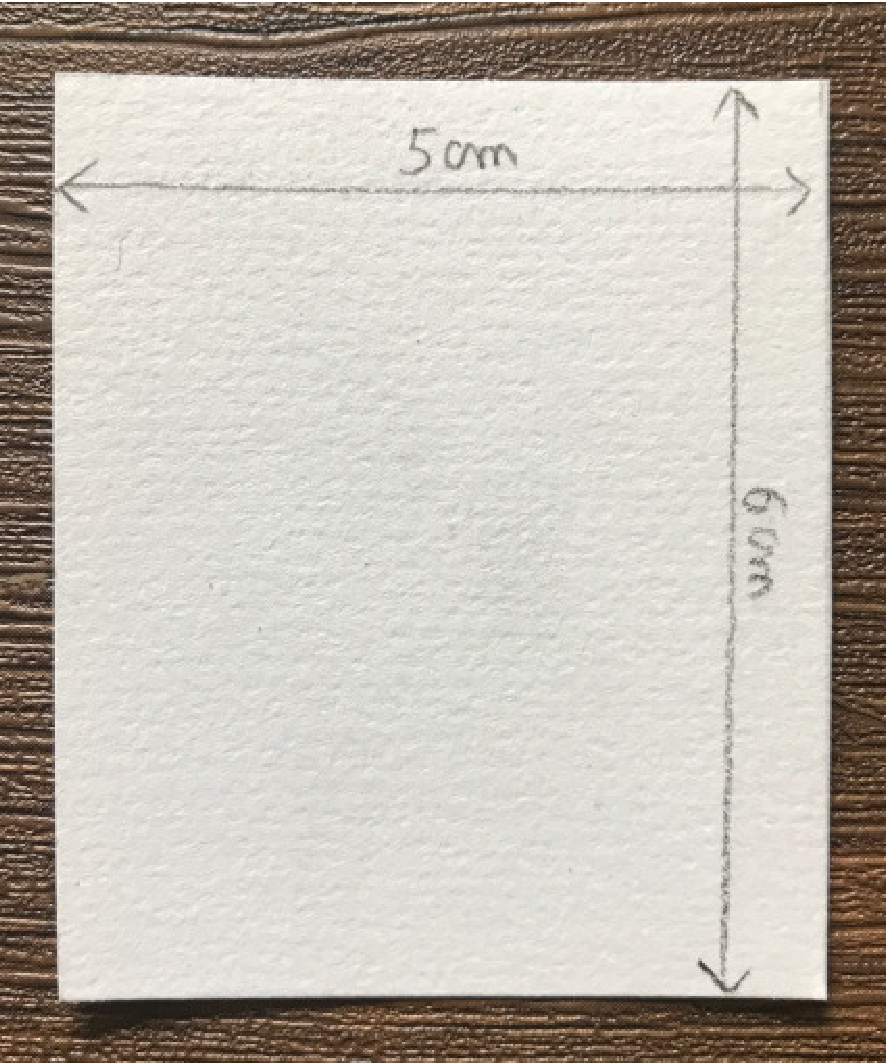
\includegraphics[width=5cm]{pavage1}
      \end{minipage}
      \qquad
      \begin{minipage}{5cm}
         \begin{enumerate}
            \item Découper dans une feuille de papier Canson un rectangle de \ucm{5} sur \ucm{6}. \smallskip
            \item Plier le rectangle en deux dans le sens de la largeur et placer trois petits bouts de scotch sur les trois côtés qui ne sont pas attachés. \smallskip
            \item Dessiner une forme qui ressemble à un poisson en deux morceaux.
         \end{enumerate}
      \end{minipage}
      \qquad
      \begin{minipage}{5cm}
         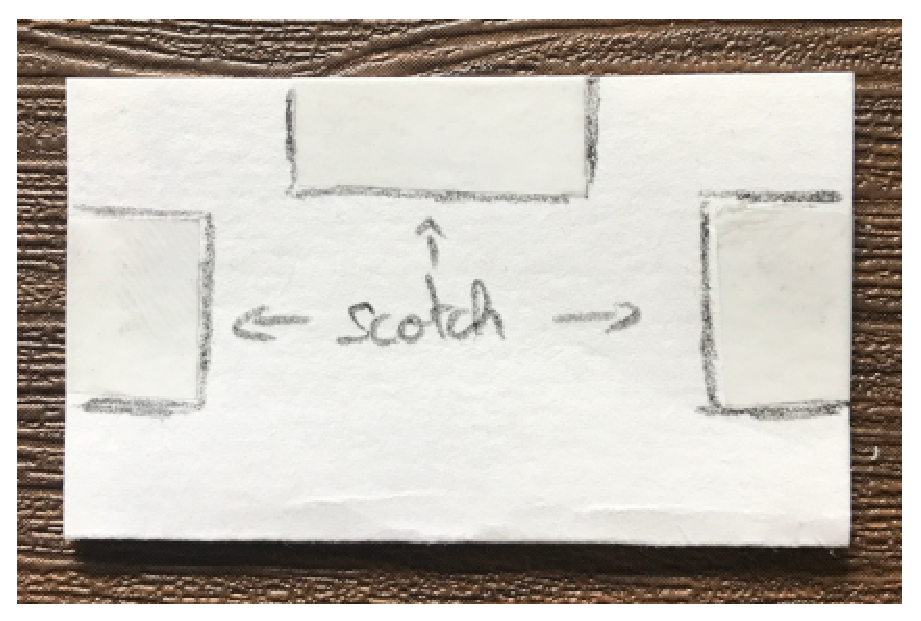
\includegraphics[width=5cm]{pavage2}
         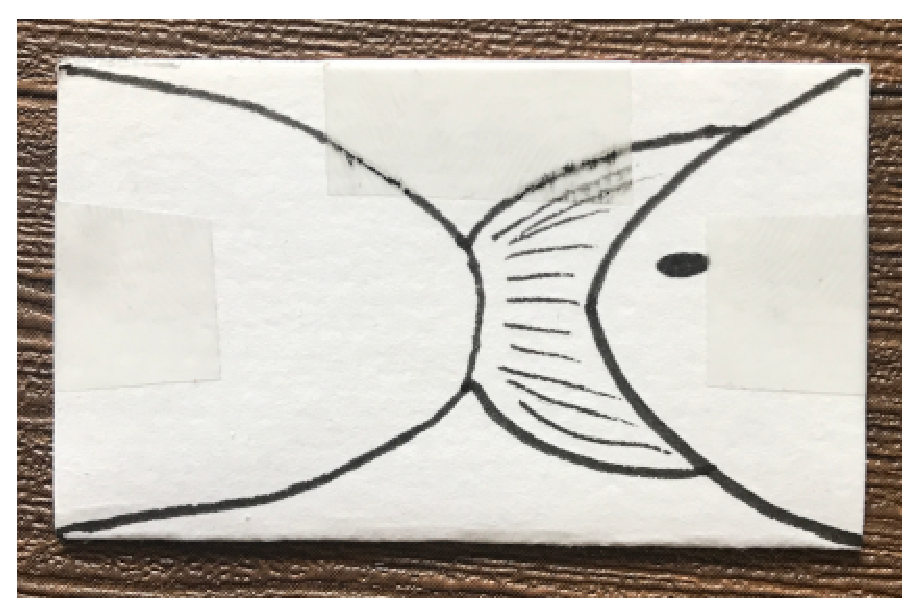
\includegraphics[width=5cm]{pavage3}
      \end{minipage} \\ \medskip
      \begin{minipage}{7cm}
         \begin{enumerate}
            \setcounter{enumi}{3}
            \item Découper selon les traits en commençant par les coins laissés sans scotch puis ouvrir afin d'obtenir la forme du poisson. \smallskip
            \item Grâce à ce gabarit, dessiner un pavage de poissons sur une feuille unie en passant de l'un à l'autre par symétrie centrale de manière à remplir toute la feuille.
         \end{enumerate}
       \end{minipage}
      \qquad
      \begin{minipage}{9cm}
         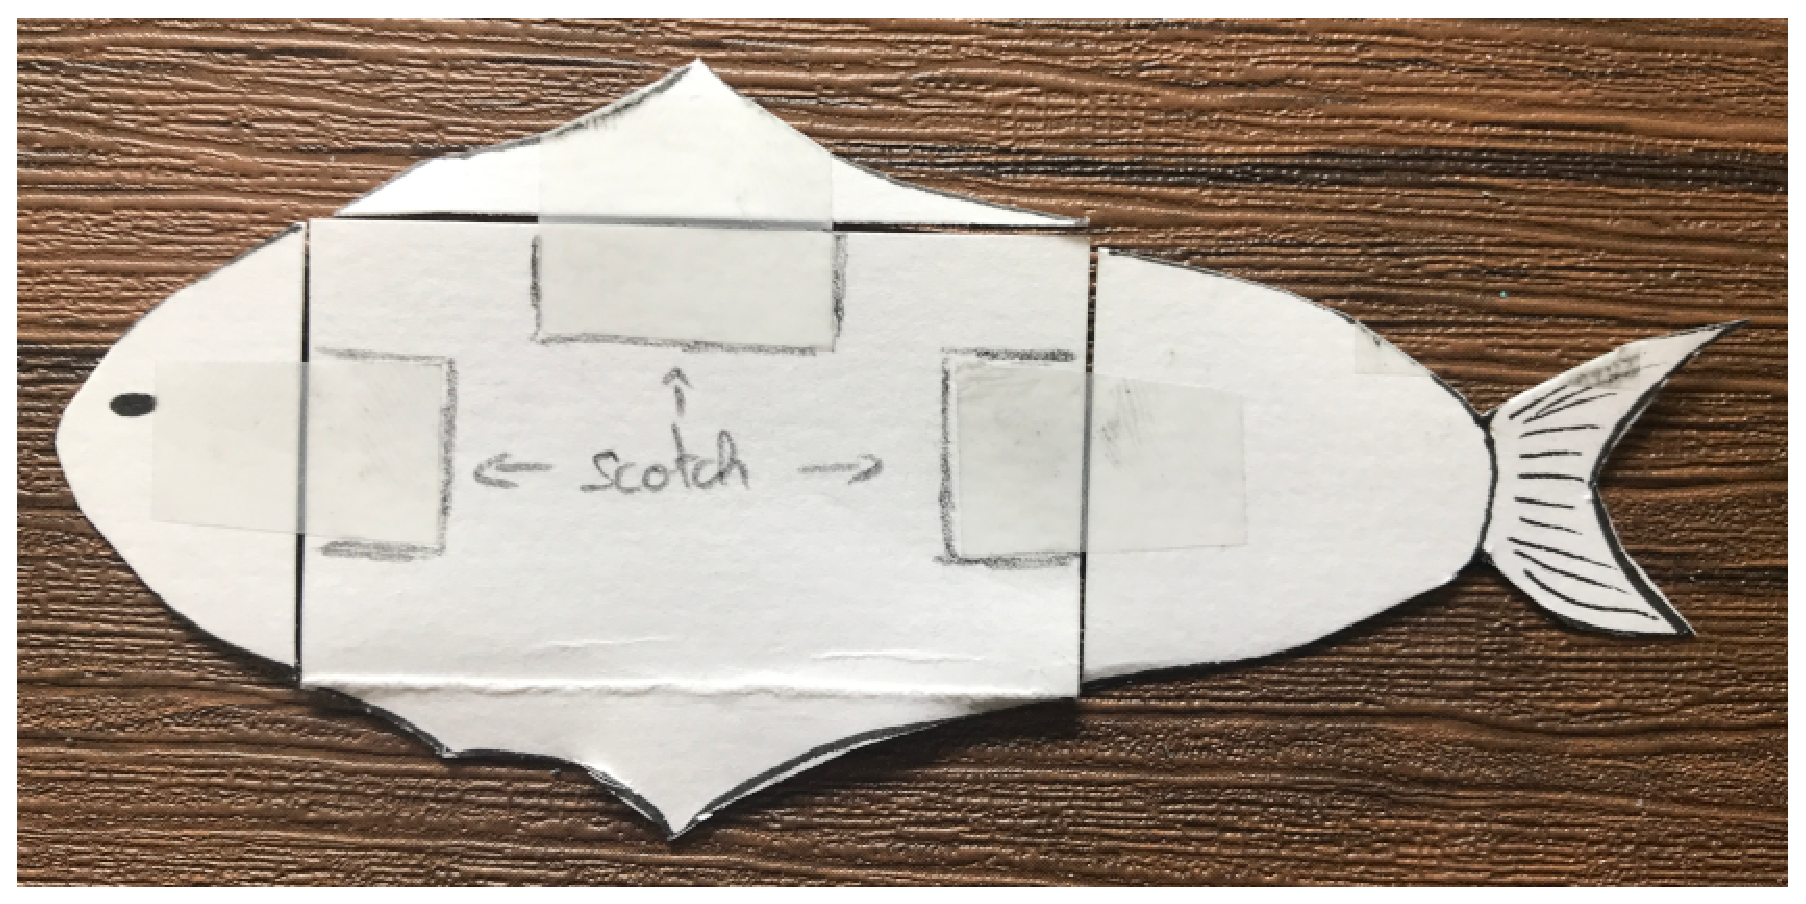
\includegraphics[width=8cm]{pavage4} 
      \end{minipage}
      \ \\ [5mm]
      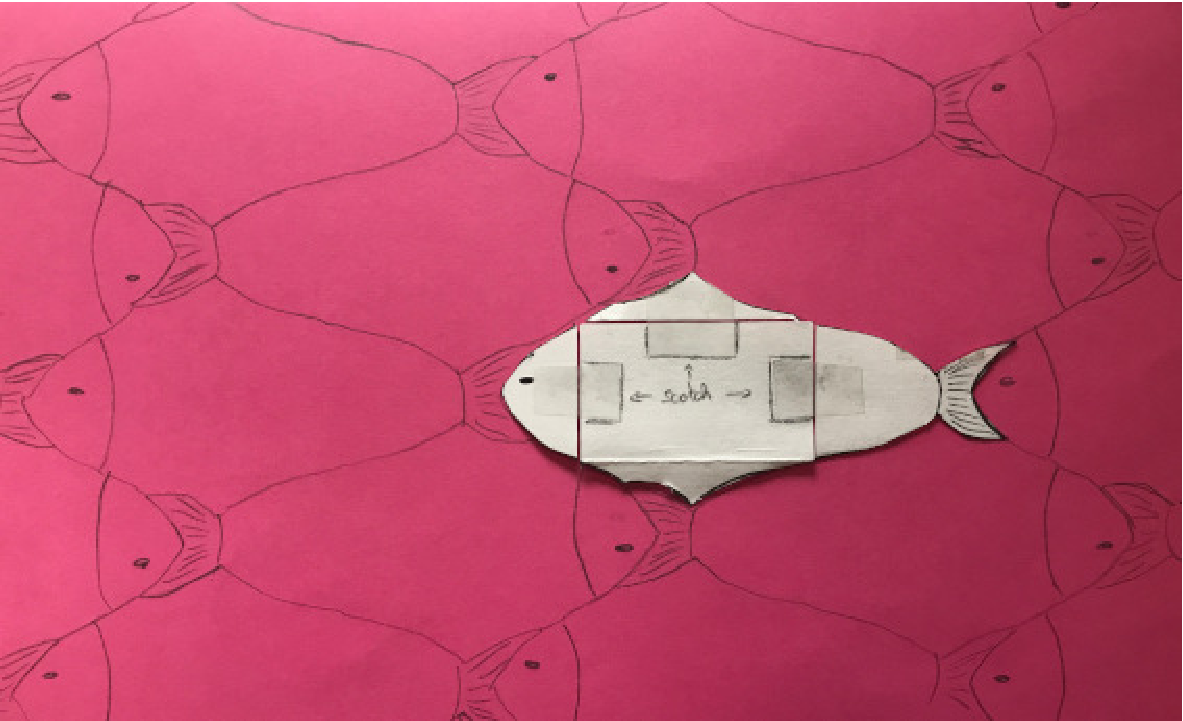
\includegraphics[width=14cm]{pavage5}
   \end{center}
 
